\documentclass[tikz]{standalone}

\begin{document}
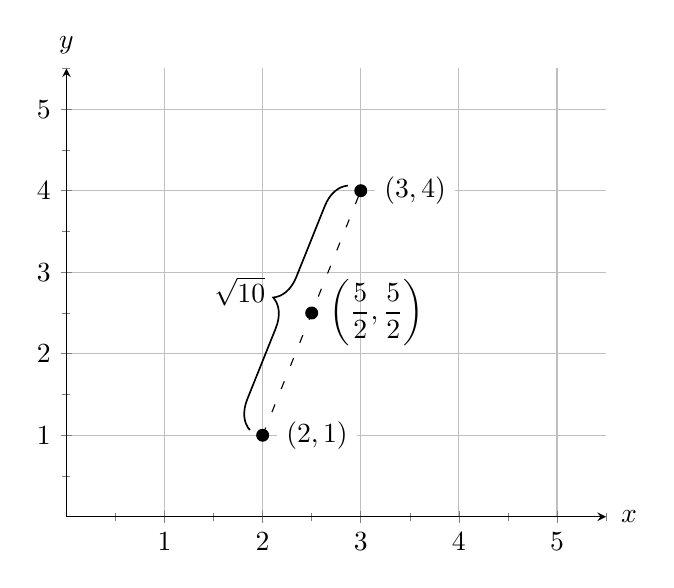
\begin{tikzpicture}
    \begin{axis}[%
        xlabel=$x$, ylabel=$y$, legend pos=south east,
        grid=major, xmin=0, xmax=5.5, ymin=0, ymax=5.5,
        axis lines = middle,
        minor x tick num=1, minor y tick num=1,
        xlabel style = {at={(axis description cs:1.01,0)},anchor=west},
        ylabel style = {at={(axis description cs:0,1.01)},anchor=south},
    ]
    \draw[black, fill=black] (2,1) circle [radius=0.75mm] node[right, fill=white, xshift=5pt]{$(2,1)$}
        (3,4) circle [radius=0.75mm] node[right, fill=white, xshift=5pt]{$(3,4)$};
    \draw[thin, loosely dashed] (2,1) -- (3,4);
    \draw[black, fill=black] ({5/2},{5/2}) circle [radius=0.75mm] node[right, xshift=3pt]{$\displaystyle \left(\frac{5}{2},\frac{5}{2}\right)$};
    \draw[semithick, decorate, decoration={brace,amplitude=10pt,mirror,raise=5pt}] (3,4) -- (2,1) node[midway, above,yshift=-1pt, xshift=-26pt]{$\sqrt{10}$};
    \end{axis}
\end{tikzpicture}
\end{document}
